\chapter{Método de elementos de borde.}\label{sec:BEM.}
\setcounter{figure}{0}
\setcounter{equation}{0}
El método de elementos de borde o BEM por sus siglas en inglés Boundary Element Method, es en escencia un método númerico para la resolución de ecuaciónes diferenciales, es muy utilizado en mecánica de fluidos, acústica, electromagnética, entre otras áreas. Cuando leemos esta definición es inevitable pensar en el método de elementos finitos o FEM, el cúal es el modelo más clasico de la resolución de este tipo de ecuaciones, pero ¿en qué se diferencian?\\
Como bien sabemos, las ecuaciones diferenciales rigen una gran cantidad de fenómenos físicos. Para resolver estas ecuaciones diferenciales se realiza un proceso llamado discretización, el cual nos entrega resultados aproximados y consiste en dividir el elemento en estudio en elementos infinitesimales y basandose en las expansiones de Taylor, poder encontrar el resultado buscado. Es aquí justamente donde encontramos la primera gran diferencia entre ambos métodos:
\begin{figure}[H]
\centering
\label{fig:Discretizacion BEM y FEM}
\subfigure[Discretización utilizada en BEM.]{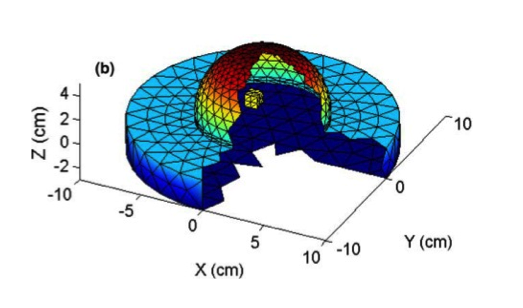
\includegraphics[height=6.8cm]{Imagenes/DiscretizacionBEM.png}}
\subfigure[Discretización utilizada en FEM.]{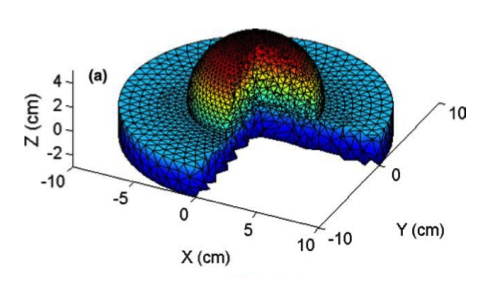
\includegraphics[height=6.8cm]{Imagenes/DiscretizacionFEM.png}}
\caption{Diferencias en la discretización en BEM y FEM en 3D.}
\end{figure}
Como observamos en la imagen, el elemento infinitesimal de estudio en FEM es un pequeño elemento de 3 dimensiones, puede ser un cubo, una piramide. Mientras que en BEM, el elemento es en 2D, triángulos, cuadrados, etc. Cabe destacar que mientras más elementos se utilicen para dividir el objeto de estudio, más preciso será el cálculo.\\
El BEM utiliza condiciones de borde o de frontera para ajustar los valores de borde a las ecuaciones diferenciales. Estás condiciones suelen ser:
\begin{equation}
\label{eq:Condiciones iniciales}
\begin{split}
\textnormal{Condiciones 'esenciales' del tipo }u=\bar{u}\textnormal{ en }\Gamma_1\\
\textnormal{Condiciones 'naturales' del tipo }q=\bar{q}\textnormal{ en }\Gamma_2
\end{split}
\end{equation}
Estas condiciones usualmente son conocidas como condiciones de Dirichlet, las condiciones 'esenciales', mientras que las condiciones 'naturales' son conocidas como condiciones de Neumann. Pueden existir condiciones de frontera más complejas tal como la combinación de las dos anteriores.\\
La ecuación integral que se usa como punto de inicio para el método es:
\begin{equation}
\label{eq:Ecuacion inicial BEM}
\nabla^2u=0
\end{equation}
Si a esta ecuación se le aplica una integral por el volumen $\Omega$ y además se multiplica por una función $w$ conveniente:
\begin{equation}
\int_\Omega\nabla^2u(r')w(r-r')\;d\Omega(r')=0
\end{equation}
Notar que estamos integrando sobre $r'$ y $r$ no está restringida. Utilizando la identidad mostrada en la ecuación \eqref{eq:Identidad gradiente} se puede descomponer de la forma :
\begin{equation}
\label{eq:Descomposicion 1}
\int_\Omega w(r-r')\nabla\cdot(\nabla u(r'))\;d\Omega(r')=\int_\Omega\nabla\cdot u(r')(\nabla w(r-r'))\;d\Omega(r')-\int_\Omega\nabla u(r')\nabla w(r-r')\;d\Omega(r')
\end{equation}
En el primer término del lado derecho de la ecuación \eqref{eq:Descomposicion 1} podemos utilizar el teorema de Gauss, indicado en la ecuación \eqref{eq:Teorema de Gauss}, mientras que en el segundo término volvemos a utilizar la identidad \eqref{eq:Identidad gradiente}, lo que nos entrega\footnote{Para facilidad de notación solo se utilizará $u$ y $w$}:
\begin{equation}
\int_\Omega \nabla^2u\;w\;d\Omega=\int_\Gamma n\cdot u\nabla w\;d\Gamma-\int_\Omega\nabla\cdot(w\nabla u)d\Omega-\int_\Omega v\nabla\cdot\nabla u\;d\Omega
\end{equation}
\begin{figure}[H]

\centering
\subfigure[Hemisfera alrededor de $i$]{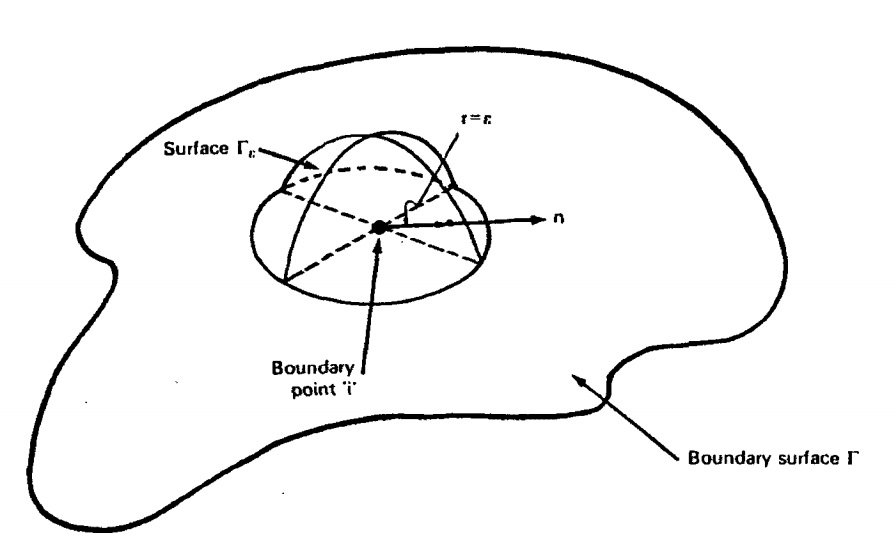
\includegraphics[scale=0.35]{Imagenes/2.2.jpg}}
\subfigure[Semicirulo alrededor de $i$]{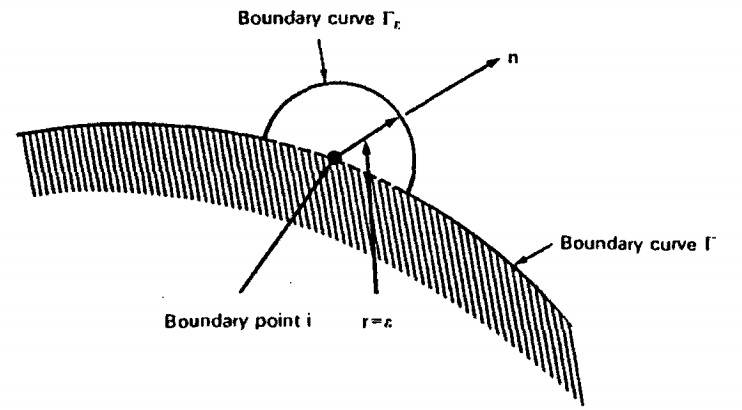
\includegraphics[scale=0.35]{Imagenes/2.3.jpg}}
\caption{Puntos de frontera para los casos 2D y 3D (Fuente:\cite{Brebbia})}\label{fig:Singularidades}
\end{figure}
Nuevamente podemos utilizar el teorema de Gauss con el segundo término del lado derecho de la ecuación. Además, igualamos la ecuación a cero tal como en \eqref{eq:Ecuacion inicial BEM}:
\begin{equation}
0=\int_\Gamma n\cdot u\nabla w\;d\Gamma-\int_\Gamma n\cdot w\nabla u\;d\Gamma-\int_\Omega u \nabla^2 w\;d\Omega
\end{equation}
Ahora llamaremos a nuestra función $w$ conveniente la solución fundamental de la ecuación, la cual tiene por segunda dervada la función Delta Dirac, la que si se encuentra bajo el dominio de la solución de la función tiene por valor 1, como este es el caso se puede afirmar que el tercer término de la ecuación tiene por valor $u(r)$. Sin embargo también hay que recordar que la función $w$ está evaluada en $(r-r')$ por lo que hay una singularidad que ocurre cuando $r\rightarrow r'$ que se debe estudiar. Esta singularidad, que está ilustrada en la figura \ref{fig:Singularidades}, genera un término libre de valor $-1/2\;u(r)$. Finalmente podemos escribir la ecuación como:
\begin{equation}
0=\int_\Gamma n\cdot u\nabla w\;d\Gamma-\int_\Gamma n\cdot w\nabla u\;d\Gamma+\frac{1}{2}u
\end{equation}
Tomando como nueva notación a $w=u*$. Notar que las divergencias están multiplicadas por un vector normal, por lo que el término afectado por el operador $\nabla$ se transforma en la derivada en la dirección normal. Reescribiendo llegamos a:
\begin{equation}
\label{eq:Ecuacion inicial BEM desarrollada}
\frac{1}{2}u^i+\int_\Gamma uq^*\,d\Gamma=\int_\Gamma qu^*\,d\Gamma
\end{equation}
En donde $u$ es una función potencial, $q$ es su derivada con respecto a la normal. $u^*$ y $q^*$ son las soluciones fundamentales de ambas funciones. El superindice $i$ indica el punto de 'anclaje' o centro del círculo o hemiesfera de interés.
Estos puntos $i$ serán considerados como 'nodos'. 
Al momento de discretizar la ecuación \eqref{eq:Ecuacion inicial BEM desarrollada} nos queda de la siguiente forma:
\begin{equation}
\label{eq:Ecuacion discretizada}
\frac{1}{2}u^i+\sum_{j=1}^N\left( \int_{\Gamma_j} q^*\,d\Gamma\right)u^j=\sum_{j=1}^N \left(\int_{\Gamma_j} u^*\,d\Gamma \right)q^j
\end{equation}
Las integrales mostadas, se llamarán para simplificar:
\begin{equation}
\label{eq:Descripcion de matriz H y G}
\hat{H}^{ij}=\int_{\Gamma_j}q^*\,d\Gamma\qquad\textnormal{ y }\qquad G^{ij}=\int_{\Gamma_j}u^*\,d\Gamma
\end{equation}	 
\begin{figure}[H]
\label{fig:Tipo de elemento de frontera}
\centering
\subfigure[Elementos constantes.]{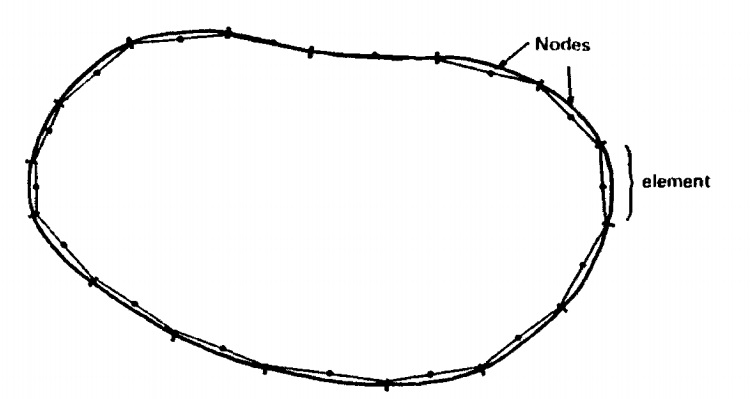
\includegraphics[scale=0.35]{Imagenes/elementos constantes.jpg}}
\subfigure[Elementos lineales.]{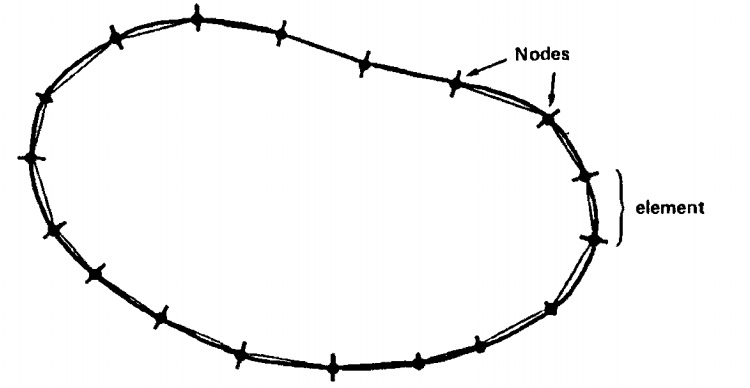
\includegraphics[scale=0.35]{Imagenes/elementos lineales.jpg}}
\subfigure[Elementos cuadráticos.]{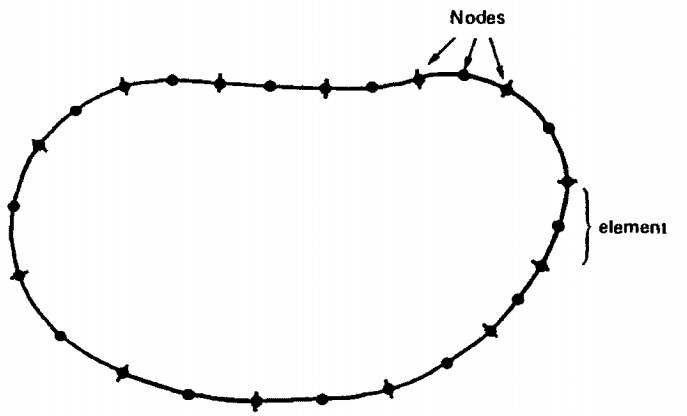
\includegraphics[scale=0.35]{Imagenes/elementos cuadraticos.jpg}}
\caption{Diferentes tipos de elementos de frontera. (Fuente:\cite{Brebbia})}
\end{figure}
\begin{equation*}
\label{eq:Desarrollo de H}
\left.
\begin{aligned}
\textnormal{Si }i\not = j&\textnormal{ entonces } \hat{H}^{ij}\\
\textnormal{Si }i\not = j&\textnormal{ entonces } \hat{H}^{ij}+\frac{1}{2}
\end{aligned}
\right\}
=H^{ij}
\end{equation*}
Entonces la ecuación \eqref{eq:Ecuacion discretizada} puede ser escrita como:
\begin{equation}
\label{eq:Sumatoria de H y G}
\sum_{j=1}^NH^{ij}u^j=\sum_{j=1}^N G^{ij}q^j
\end{equation}
Esta serie de ecuaciones puede ser expresada en forma de matriz como:
\begin{equation}
\label{eq:Forma matricial HU=GQ}
HU=GQ
\end{equation}
Podemos llevar todos los términos conocidos al lado izquierdo y los valores iniciales conocidos (como los ejemplificados en la ecuación \eqref{eq:Condiciones iniciales}), reescribiendola como:
\begin{equation}
\label{eq:Forma matricial AX=F}
AX=F
\end{equation}
Entonces, si nuestras condiciones iniciales son solo de Dirichlet, el vector $X$ estaría compuesto solo por 'valores desconocidos' de $q$ y viceversa. Si fuera una mezcla de ambas condiciones, el vector $X$ sería una mezcla de $u's$ y $q's$, evidentemente luego deberían reordenarse los valores y dejar un solo vector de $u's$ y otro distinto para $q's$. Esto es consecuencia de la formulación mixta de elementos de frontera y entrega una importante ventada respecto a elementos finitos.
\begin{figure}[H]
\label{fig:Discretizacion BEM y FEM 2}
\centering
\subfigure[Discretización utilizada en BEM.]{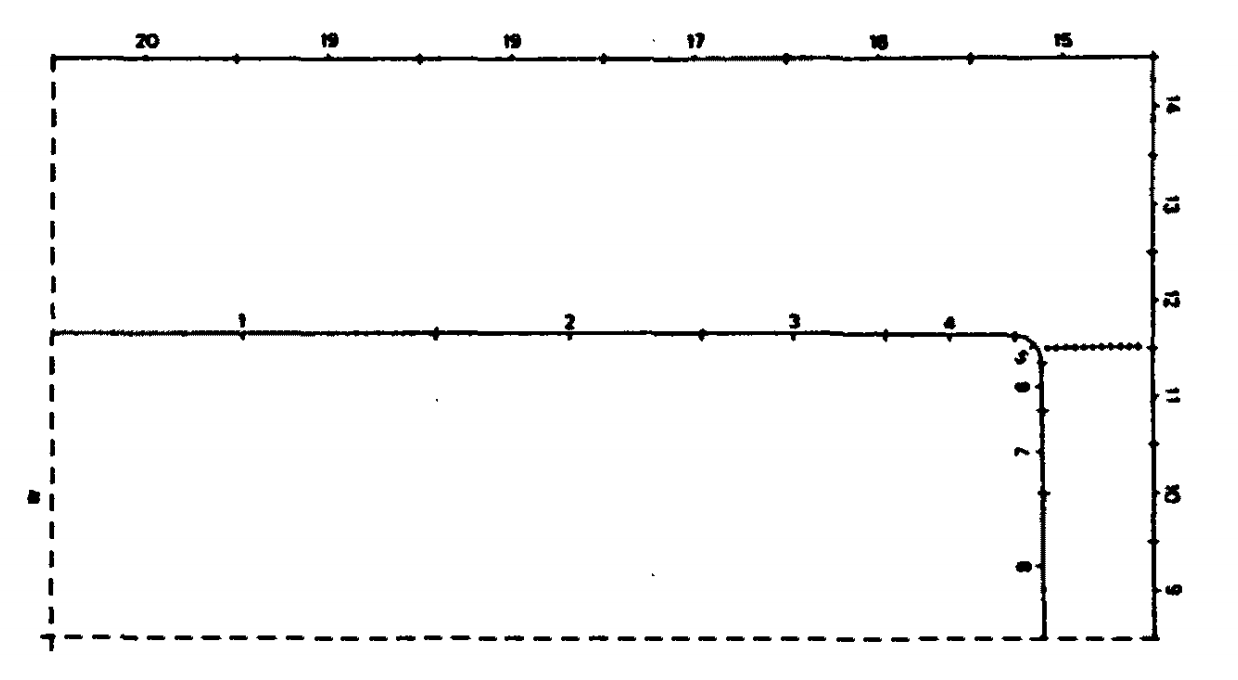
\includegraphics[height=6.8cm]{Imagenes/disbem.png}}
\subfigure[Discretización utilizada en FEM.]{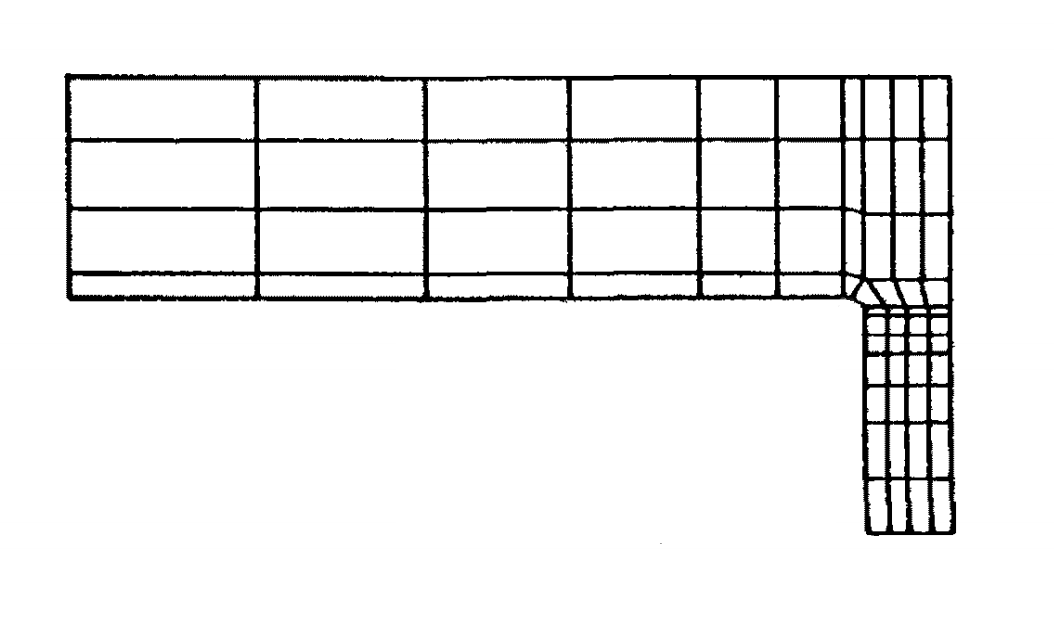
\includegraphics[height=6.8cm]{Imagenes/disfem.png}}
\caption{Diferencias en la discretización en BEM y FEM en 2D  (Fuente:\cite{Brebbia}).}
\end{figure}
Es necesario hacer un par de alcances, para comprender mejor lo explicado anteriormente:
Las integrales mostradas en la ecuación \eqref{eq:Descripcion de matriz H y G} son resueltas mediante una cuadratura de Gauss, la cual es una aproximación de la integral. En el problema a resolver en este informe, se utiliza una cuadratura con 4 nodos.\\
Es importante indicar que BEM es aplicable a problemas que puedan ser modelados por una función de Green, ya sea Laplace, Helmholtz o Helmholtz modificado. Es necesario hacer notar que las funciones de Green son principalmente utilizadas para modelar ecuaciones diferenciales con condiciones de contorno dadas, que es justamente como hemos definido los problemas de BEM.
\newpage
¿Qué sucede con los puntos internos? Como dijimos en un principio, el comportamiento en el interior del cuerpo de estudio es homogeneo, por lo tanto es posible hacer una buena aproximación o predicción de como se comportará la función potencial estudiada en el cuerpo en los puntos interiores. Gráficamente los puntos interiores serían algo como:
\begin{figure}[H]
\centering
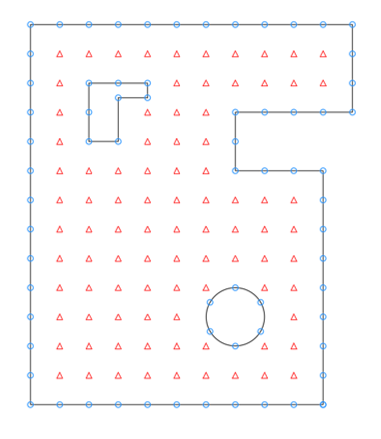
\includegraphics[scale=1]{Imagenes/bem.png}
\caption{Elementos de borde y puntos internos para el estudio}\label{fig:Puntos internos de BEM}
\end{figure}
Para calcular el potencial es necesario utilizar la ecuación que se muestra a continuación. Es necesario hacer notar que los coeficientes $H^{ij}$ y $G^{ij}$ son recalculados para cada punto interno. 
\begin{equation}
\label{eq:Calculo puntos internos discretizada}
u^i=\sum_{j=1}^NG^{ij}q^j-\sum_{j=1}^N\hat{H}^{ij}u^j
\end{equation}
El cálculo para la derivada en ambas direcciones en los puntos internos también se puede realizar, pero su formulación es como sigue:
\begin{equation}
\label{eq:Calculo derivada en puntos internos}
\begin{split}
\left(q_{x_1}\right)=\left(\frac{\partial u}{\partial x_1}\right)^i=\sum_{j=1}^N\left(\int_\Gamma \frac{\partial u^*}{\partial x_1}\,d\Gamma\right)q^j-\sum_{j=1}^N\left(\int_\Gamma \frac{\partial q^*}{\partial x_1}\,d\Gamma\right)u^j\\
\left(q_{x_2}\right)=\left(\frac{\partial u}{\partial x_2}\right)^i=\sum_{j=1}^N\left(\int_\Gamma \frac{\partial u^*}{\partial x_2}\,d\Gamma\right)q^j-\sum_{j=1}^N\left(\int_\Gamma \frac{\partial q^*}{\partial x_2}\,d\Gamma\right)u^j\\
\end{split}
\end{equation}